\documentclass[10pt]{standalone}
\input{../../tikzpic_packages.tex}

\begin{document}
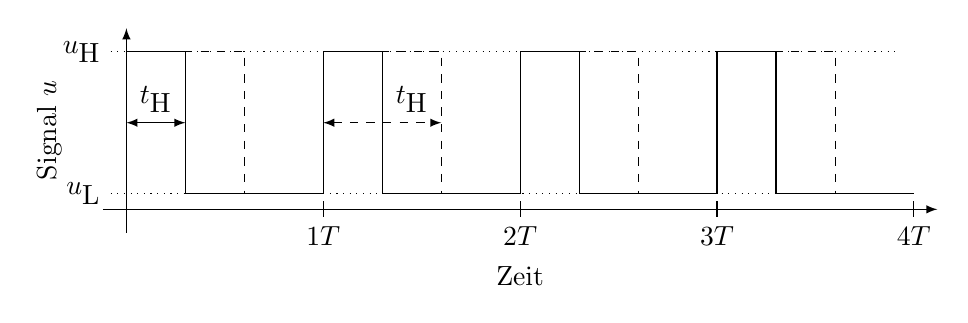
\begin{tikzpicture}[
scale = 1,
block/.style={draw, rectangle, minimum height=1cm, minimum width=1cm},
bigblock/.style={draw, rectangle, minimum height=1cm, minimum width=2cm},
sum/.style={draw, circle, inner sep=0pt, minimum width=.2cm},
connect/.style={draw, circle, fill, inner sep=0pt, minimum width=.05cm},
arrow/.style={-latex}
]
\def\xaxl{10}
\def\yaxl{2}
\def\T{2.5}

\pgfmathsetmacro{\high}{\yaxl}
\pgfmathsetmacro{\low}{.2}
\pgfmathsetmacro{\mid}{.5*(\high+\low)}



\draw[arrow] (-.3,0)--(\xaxl+.3,0)node[midway, below=.6cm]{Zeit};
\draw[arrow] (0,-.3)--(0,\yaxl+.3)node[midway, sloped, above=.7cm]{Signal $u$};

\draw[dotted] (-.2,\high)node[left]{$u_{\textnormal{H}}$}--++(\xaxl,0);
\draw[dotted] (-.2,\low)node[left]{$u_{\textnormal{L}}$}--++(\xaxl,0);

\def\pwm{.3}
\pgfmathsetmacro{\ende}{\xaxl-\T}
\foreach[count = \i] \x in {0,\T,...,\ende}{
	\pgfmathsetmacro{\dx}{\T*\pwm}
	\draw (\x,\low)--(\x,\high)--(\x+\dx,\high)--(\x+\dx,\low)--(\x+\T,\low);
	\ifnum\i>0	\draw (\x+\T,.1)--++(0,-.2)node[below]{\i $T$}; \fi
	\ifnum\i=1 \draw[latex-latex] (\x,\mid)--++(\dx,0)node[midway, above]{$t_{\textnormal{H}}$}; \fi
}

\def\pwm{.6}
\pgfmathsetmacro{\ende}{\xaxl-\T}
\foreach[count = \i] \x in {0,\T,...,\ende}{
	\pgfmathsetmacro{\dx}{\T*\pwm}
	\draw[dashed] (\x,\low)--(\x,\high)--(\x+\dx,\high)--(\x+\dx,\low)--(\x+\T,\low);
	\ifnum\i=2 \draw[latex-latex, dashed] (\x,\mid)--++(\dx,0)node[pos=.75, above]{$t_{\textnormal{H}}$}; \fi
}

\end{tikzpicture}
\end{document}